\documentclass[11pt]{article}

\usepackage[english]{babel}
\usepackage[utf8]{inputenc}
\usepackage[T1]{fontenc}
\usepackage{lmodern}
\usepackage{geometry}
\geometry{a4paper, margin=2.5cm}

\usepackage{graphicx}
\usepackage{hyperref}
\usepackage{listings}
\usepackage{xcolor}

\lstdefinestyle{javaStyle}{
    language=Java,
    basicstyle=\ttfamily\small,
    keywordstyle=\color{blue}\bfseries,
    commentstyle=\color{gray}\itshape,
    stringstyle=\color{teal},
    numbers=left,
    numberstyle=\tiny\color{gray},
    stepnumber=1,
    showstringspaces=false,
    breaklines=true,
    frame=single,
    captionpos=b
}

\title{Introduction to Computer Networking\\Tic-tac-toe Project Report}

\author{Franck Duval HEUBA \\ Student ID: S227629}
\date{October 26, 2025}

\begin{document}
\maketitle

\section{Introduction}
This project involves the design and implementation of a \textbf{concurrent, text-based Tic-Tac-Toe game} using \textbf{Java TCP sockets}.
 The core task is to build a robust server that can manage multiple simultaneous clients and arbitrate games according to a well-defined 
 protocol. The server must support two distinct modes: a single-player mode where a user competes against a bot with random move logic, 
 and a multiplayer mode that pairs two clients for a head-to-head match. The client application will handle user input from the console
  and communicate with the server to play the game.

\section{Software Architecture}

\begin{figure}
    \centering
    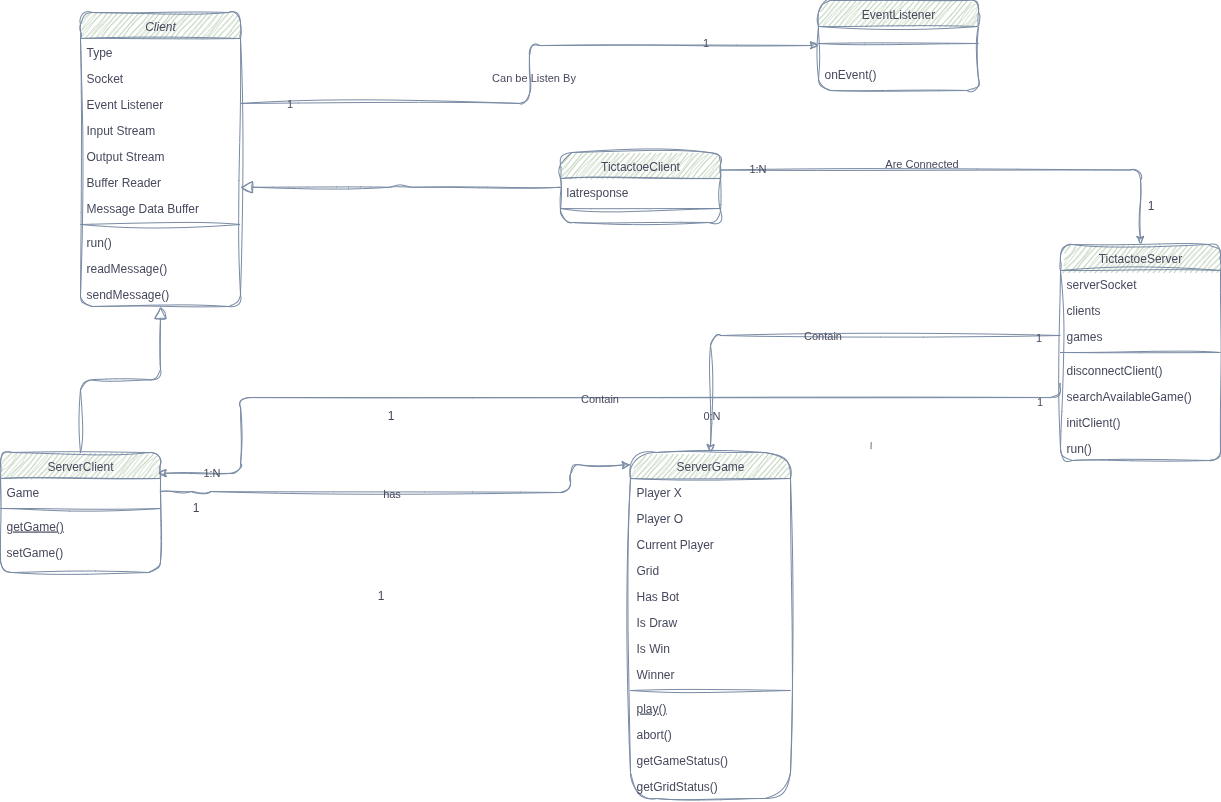
\includegraphics[width=1\textwidth]{./images/project-1.drawio.png}
    \caption{Software Architecture Diagram}
\end{figure}

There is six main classes in this project:
\begin{itemize}
    \item \textbf{Client} class: this class represent a client 
    \item A \textbf{Client} Can either a Connected Client who is using his terminal \textbf{TictactoeClient}
    \item Or a connected client on the server side \textbf{ServerClient}
    \item \textbf{ServerGame} is a game created by the server for two player either (ServerClient, Bot) or (ServerClient, ServerClient)
    \item \textbf{TictactoeServer} is the main server class which handle all the connections and create games
    \item \textbf{EventListener} interface is used to handle events between classes
\end{itemize}

First the \textbf{TictactoeServer} is started and listen for incoming connections. When a user want to play, 
a \textbf{TictactoeClient} is created to handle the communication with the server.
The \textbf{TictactoeClient} will listen for messages from the server and handle them accordingly.
The user can then choose to play against a bot or against another player then other instructions.
When a client connect (server side) a new \textbf{ServerClient} is created to handle the communication with this client.
The \textbf{ServerClient} will listen for messages from the client and handle them accordingly.
When a client want to start a game, the \textbf{TictactoeServer} will create a new \textbf{ServerGame} for this client.
If the client want to play against a bot, the \textbf{ServerGame} will set-up the internal bot of the \textbf{ServerGame} classes then start the game.
If the client want to play against another client, the \textbf{TictactoeServer} will wait for another client to connect and then start the game.    

\newpage

Another very important classes but not present in the Diagram is \textbf{TictactoeResponse} which is used to handle the messages between the client and the server.
A message send by the \textbf{TictactoeClient} will be received on the server side by the \textbf{ServerClient} and inversely. When a message is received, if the 
\textbf{Client(TictactoeClient or ServerClient)} possess an \textbf{EventListener} it will call the appropriate method to handle the message \textbf{onEvent(response)}.
Any received message is a \textbf{response(text)} which is parsed with a \textbf{TictactoeResponse} object by his own constructor. The \textbf{TictactoeResponse} contains all data of the response.


\section{Program logic}

The logic of our \textbf{TictactoeServer} is quiet simple.

\begin{itemize}
    \item The main loop is running until the server is stopped by a \textbf{Ctrl+C} command or by a defect in the code (which should not normally happen).
    \item Each iteration of the loop will check for new incoming connections.
    \item When a new connection is established, a new \textbf{ServerClient} is created to handle the communication with this client (\textbf{TictactoeClient}) and added to the client's list.
    \item When a \textbf{ServerClient} when a dedicted thread is created to manger all possible operatios with this client.
    \item A \textbf{EventListener} is attached to the \textbf{ServerClient} to handle all incoming messages from this client (the methode initClient).
    \item when a message is received from the client, the appropriate method of the \textbf{EventListener} is called to handle the message (onEvent).
    \item The text message is parsed with a \textbf{TictactoeResponse} object to extract all data of the message.
    \item Depending on the type of message, the appropriate action is taken (start game, make move, etc).
    \item When the client want to start a game, a new \textbf{ServerGame} is created for this client.
    \item A ServerGame is always added to the list of games in the server.
\end{itemize}


\section{TCP Stream}
When a \textbf{Client (TictactoeClient or ServerClient)} is created the started method is called.
the main loop of the client is running until the client is disconnected. Using \textbf{BufferedReader}, 
which is created in the construcor with \textbf{InputStreamReader} and \textbf{InputStream}, the main loop
of the client will call \textbf{readLine()} method to read a line from the buffer reader.
When a line is received, $total\_message = temp + received$, where temp is a part of the message which have been received previously.
Then we check if the $total\_message$ contains the end of message character \texttt{\textbackslash r\textbackslash n} If it does, if the end character is at the end of the message,
we will split the $total\_message$, then for each part we will give it to the \textbf{TictactoeResponse} constructor to parse it.
If the end character is not at the end of the message, we split the message in multiple, the we parse each message with a \textbf{TictactoeResponse} constructor.
excepted for the last part of the message which is stored in temp for the next iteration.
\vspace{10px}

When a \textbf{TictactoeResponse} is created, the constructor will use two regex to validate the message.
is follow the Tic Tac Toe protocol. The first regex is used to validate the command part of the message,
and the second regex is used to validate the puzzle part of the message (if present).

if the received message is neither a valid command nor a valid puzzle, an \textbf{TictactoeResponseException} is thrown.

\begin{lstlisting}[style=javaStyle, language=Java, caption={Response parsing in TictactoeResponse}]
    // command_regex
    Pattern.compile("^([A-Z]+)(\\s+[A-Z]{2,})?(\\s+[A-Z]{2,})?(\\s+[A-Za-z]|\\s+\\-?[0-9]+)?(\\s+[A-Za-z]|\\s+\\-?[0-9]+)?\\s*\\r\\n(\\r\\n)?$");

    // puzzle_regex
    Pattern.compile("^([XxOo\\s]{3}\\r\\n){3}(([XxOo] WON|DRAW|OPPONENT QUIT)\\r\\n)?(\\r\\n)?$");
\end{lstlisting}

\section{Multi-threading}
Yes my server server enable multiple games (single and multiplayer) to be played simultaneously without interfering with each other.
A \textbf{ServerGame} is a game between two players (ServerClient, Bot) or (ServerClient, ServerClient). Each \textbf{ServerGame} and each 
client are store in a dedicted list in the \textbf{TictactoeServer} class. \newline
A game is a shared object which can only by acceded by the two players (ServerClient) maximun. \newline
The main Thread (TictactoeServer) is alone to access to the list of clients and the list of games.

When a client is deconnected, \textbf{ServerClient} thrown an exception which is catched by the server object.

\section{Robustness}
My server is robust because it use the concept of exceptions to handle errors and atomicity.
When an error occur, or a bad state, the appropriate exception is thrown by the current class, 
and catched by the class above. Each class is responsible to handle its own errors and to throw the appropriate exception.
For example, when a \textbf{TictactoeResponse} is created, if parameters(a message from the client or the server) are not valid, a \textbf{TictactoeResponseException} is thrown.
This exception is catched by the \textbf{ServerClient} or the \textbf{TictactoeClient} class which will handle the error accordingly (send an error message to the other side, disconnect the client, etc).
This way, each class is responsible to handle its own errors and to throw the appropriate exception.

\section{Conclusion}
\begin{itemize}
    \item The most challenging is to catch all possible errors and to handle them accordingly to the context.
    \item It was the first time I used mutti-threading in Java, so I had to learn how to use it properly.
    \item I learned how to use Java sockets to create a TCP server and client.
    \item I learned how to use regex to validate and parse messages.
    \item I learned how to use exceptions to handle errors and to make my code more robust
\end{itemize}

\end{document}
